\section{Mechanical modeling}
\label{sec:intro_mechanical}

In this section we will cover the necessary theory of continuum
mehcanics in order to model the mechanics of the heart. The theory of
continuum mechancs is exstensive, and we will not be able to cover
everything. For a complete review of continuum mechanics the reader is
therefore referred the textbook of Gerard Holzapel
\cite{holzapfel2000nonlinear} from which most of the theory in this
section is taken. For the even more mathematically oriented reader we
refer to \cite{marsden1994mathematical}.

We represent the heart as a continuum body $\mathfrak{B}$ embedded in
$\mathbb{R}^3$. A configuration of $\mathfrak{B}$ is a mapping $\chi:
\mathfrak{B} \rightarrow \mathbb{R}^3$. 
We denote the \emph{reference configuration} of the heart by $\Omega_0
\equiv \chi_0(\mathfrak{B})$, and the \emph{current configuration} by $\Omega
\equiv \chi(\mathfrak{B})$. The mapping $\varphi :  \Omega_0
\rightarrow \Omega$ given by the composition $\varphi = \chi
\circ \chi_0^{-1}$ is a smooth, orientation preserving (posive
determinant) and invertible map. We denote the coordinates in the
referece configuration by $\Xvec \in \Omega_0$, and the coordinates in the current
configuration by $\xvec \in \Omega$. The coordinates $\Xvec$ and $\xvec$ are
commonly refered to as material and spatial points respectively, and
are related throgh the mapping $\varphi$, by $\xvec = \varphi(\Xvec)$.
For time-dependent problems it is common to make  the time-dependence
explicitely by writing $\xvec = \varphi(\Xvec, t)$. In the following
we will only focus on the mapping between two configurations and
therefore no time-dependence is needed. The mapping $\varphi$ will be
referred to as the \emph{motion}. The \emph{deformation gradient} is a
rank-2 tensor, defined as the partial derivative of the motion with
respect to the material coordinates:
\begin{align}
  \F(\Xvec) = \frac{\partial \varphi}{\partial \Xvec} = \Grad \xvec.
  \label{eq:deformation_gradient}
\end{align}
Here we also introduce the notation $\Grad$, which means derivative
with respect to reference coordinates.
The deformation gradient maps vectors in the referece configuration to
vectors in the current configuration, and belongs to the space of
linear transformations from $\mathbb{R}^3$ to $\mathbb{R}^3$ with
strictly posive determinant, which we denote by
$\mathrm{Lin}^+$. Another important quantity is the
\emph{displacement} field  
\begin{align}
  \uvec = \xvec-\Xvec, 
  \label{eq:displacement}
\end{align}
which relates postitions in the reference configuration to positions
in the current configuration. From \eqref{eq:deformation_gradient} we
see that
\begin{align}
  \F = \Grad \xvec = \Grad \uvec + \Grad \Xvec = \Grad \uvec + \I
\end{align}
Some other useful quantities are the \emph{right Cauchy-Green} deformation
tensor $\C = \F^T\F$, the \emph{left Cauchy-Green} deformation tensor
$\mathbf{B} = \F\F^T$, the \emph{Green-Lagrange} strain tensor
$\mathbf{E} = \frac{1}{2}(\C - \I)$, and the determinant of the
deformation gradient $J = \det \F$.

An important concept in mechanics is the concept of stress, which is
defined as force per area
$\left[\frac{\mathrm{N}}{\mathrm{m}^2}\right]$. When working with
different configurations one needs to be careful with which forces and
which areas we are talking about. Table \ref{tab:stress_tensor}
shows how forces and areas are related for the most important stress
tensors used in this thesis.  

\begin{table}[h]
  \centering
  \begin{tabular}{lll}
    \toprule
    Stress tensor & Forces & Area \\
    \midrule
    Second Piola-Kirchhoff ($\SPK$) & Referece configuration & Referece configuration \\
    First Piola-Kirchhoff ($\FPK$) & Current configuration  &  Referece configuration \\
    Cauchy ($\Cauchy$) &  Current configuration & Current configuration  \\
    \bottomrule
  \end{tabular}
  \caption{\label{tab:stress_tensor}Different stress tensor, and how
    they relate forces to areas though different configurations.}
\end{table}


Perhaps a word about stress-strain work conjugates?

\subsection{Balance laws and trasformations}

\subsubsection{Transformations between reference and current
  configuration}
By definition the reference configuration, $\Omega_0$ and current
configuration $\Omega$ are related via the motion $\varphi$ in the
sense that a point $p$ with reference coordinates $\Xvec$ and current
coordinates $\xvec$ satisfies $\xvec = \varphi(\Xvec)$. Likewise a
vector in the $\Omega_0$ is related to a vector in $\Omega$ via the
deformation gradient $\F$; if $\mathrm{d}\Xvec$ is a vector in the
reference configuration it will transform to the vector
$\mathrm{d}\xvec$ in the current cofiguration, and $\mathrm{d}\xvec =
\F \mathrm{d}\Xvec$. From this relation we also derrive that the
transformation of an infinitesimal volume element in the reference
cofiguration, $\mathrm{d}V$ is related to an infinitesimal volume
element in the current cofiguration, $\mathrm{d}v$  via the determinant of the
deformation gradient,
\begin{align}
  \mathrm{d}v =\det(\F) \mathrm{d}V.
  \label{eq:volume_element}
\end{align}
Another important transformation is the transformation of normal
vectors. By noting that we can write \eqref{eq:volume_element} using
surface elements
\begin{align*}
  \mathrm{d}s \mathbf{n} \mathrm{d}\xvec  &= \mathrm{d}v = \det(\F) \mathrm{d}V = \det(\F) \mathrm{d}S  \Nvec \mathrm{d}\Xvec\\
  &\implies \left( \mathrm{d}s \mathbf{n} \F  - \mathrm{d}S \det(\F) \Nvec \right) \mathrm{d}\Xvec = 0\\
  &\implies \left( \mathrm{d}s \F^T \mathbf{n}  - \mathrm{d}S \det(\F) \Nvec \right) \mathrm{d}\Xvec = 0,\\
\end{align*}
we get \emph{Nanson's formula}
\begin{align}
  \mathrm{d}s \mathbf{n}  =  \det(\F) \F^{-T} \mathrm{d}S \Nvec,
\end{align}
which related normal vector in the current configuration to normal
vector in the reference configuration.


\subsubsection{Conservation of linear momentum}
Newton's seconds law states that the change in linear momentum equals
the net impulse acting on it. For a continuum materal with constant
mass density $\rho$ this implies that
\begin{align}
  \int_{\Omega} \rho \dot{\mathbf{v}} \mathrm{d}v = \mathbf{f},
  && \mathbf{f} = \int_{\partial \Omega} \mathbf{t} \mathrm{d}s
     + \int_{\Omega} \mathbf{b} \mathrm{d}v,
     \label{eq:cons_lin_mom}
\end{align}
where $\mathbf{v}$ is the spatially velocity field, $\mathbf{t}$ is
the traction acting on the boundary, and $\mathbf{b}$ is the body
force. From \emph{Cauchy's stress theorem} we know that there exist a
second order tensor $\sigma$, known as as Cauchy stress tensor that is
related to the traction vector by $\mathbf{t} = \sigma \mathbf{n}$,
where $\mathbf{n}$ is the unit normal in the current configuration.
Using the divergence theorem we get.

\begin{align*}
  \int_{\partial \Omega} \mathbf{t} \mathrm{d}s
  = \int_{\partial \Omega} \sigma \mathbf{n} \mathrm{d}s
  = \int_{\Omega} \nabla \cdot \sigma \mathrm{d}v,
\end{align*}
and by collecting the terms from \eqref{eq:cons_lin_mom}. We arrive at
Cauchys momentum equation
\begin{align}
  \nabla \cdot \sigma + \mathbf{b} =  \rho \dot{\mathbf{v}}
  \label{eq:chauch_momentum_eq}
\end{align}
The contribution for the body force ($\mathbf{b}$)  and inertial term
($\rho \dot{\mathbf{v}}$) are negligible compared to the stresses
\cite{hunter1996kd,tallarida1970left}, which is why the force balance
eqautions is typically only stated as
\begin{align}
  \nabla \cdot \sigma = \mathbf{0}
  \label{eq:force_balance_strong}
\end{align}
Note that we have formulated the balance law in the current
configuration. An equivalent statement can be formulated in terms of
the reference condiguration
\begin{align}
  \nabla \cdot \FPK = \mathbf{0}, 
  \label{eq:force_balance_strong_ref}
\end{align}
where $\FPK$ is the first Piola-Kirchoff stress tensor.

\subsubsection{Conservation of angluar momentum}
Just like linear momentum, the angular momentum is also a conserved
quantity. We will not go through the derivation of resulting
eqautions, but state that as a consequense, the Cauchy stress tensor is
symmetric
\begin{align}
  \sigma = \sigma^T
\end{align}



\subsection{Hyperelasticity}
\label{sec:hyperelasticity}

Even though experimental studies have idicated a viscoelastic behavior
of the myocardium \cite{dokos2002shear, gultekin2016orthotropic}, a
common assumption is to consider a quasistatic behaviour and therefore
it is also possible to model the myocardium as hyperelastic.
This means that we postulate the existence of
a strain-energy denisity function $\Psi:\mathrm{Lin}^+ \rightarrow
\mathbb{R}^+$ which is defined as energy per unit reference volume,
and has units $\frac{\text{Joule}}{m^3}$. The first Piola-Kirchhoff
stress for a hyperelastic material is given by th relation
\begin{align}
\FPK = \frac{\partial \Psi(\F)}{\partial \F}
\end{align}
The strain-energy density function relates  the amount of
energy that is stored within the material in response to a given
strain. Hence, the stresses in a hyperelastic material with a given
strain-energy density function, depends only on the strain, and not the
path for which the material deforms. On the contrary, if the model had
been viscoelastic we would expect to see hysterisis in the
stress/strain curve, but this is not possible for a hyperelastic
material. 

We say that the strain energy should be objective, meaning that the
stored energy in the material should be invariant with respect to
chage of observer. Formally we must have for any positive symmetric
rank-2 tensor $\C \in \mathrm{Sym}$ 
\begin{align}
  \Psi(\mathbf{C}) = \Psi(\mathbf{Q}\mathbf{C}\mathbf{Q}^T), \; \forall \mathbf{Q} \in \mathcal{G} \subseteq \mathrm{Orth},
\end{align}
where $\mathrm{Orth}$ is the group of all postive orthogonal matrices.
If $\mathcal{G} = \mathrm{Orth}$ we say that the matieral is
isotropic, and otherwise we say that the material is anisotropic.
This brings us to another important issue, which is related to the
chioce of coordinate-system. Having to deal with different
coordinate-systems and mappping quantities from one coordinate-system
to another can results in complicated computation, and the chances of
doing errors are increased. Therefore if would be beneficial if we
could work with quantities which do not depend on the choice of
coordinate-system. Such quantities are called invariants, and from their
name it shold be clear that they are invariant with respect to choice
of coordinate-system. 
If the material is isotropic, the representation theorem for
invariants states that $\Psi$ can be expressed in terms of the
principleinvariants of $\mathbf{C}$, that is $\Psi = \Psi(I_1, I_2,
I_3)$. The principle invariants $I_i, i=1,2,3$ are the coefficients in
the characteristic polynomial of $\mathbf{C}$, and is given by 
\begin{align}
  I_1 = \tr \C,  && I_2 = \frac{1}{2}\left[ I_1^2 - \tr(\C^2)\right] && \text{and} && I_3 = \det \C.
\end{align}
In the case when the material constitutes a transversally isotropic
behavior, that is the material has a preferred direction $\mathbf{a}$
which in the case of the myocardium could be the direction of fiber
muscle fibers, we have
\begin{align*}
  \mathcal{G} = \{ \mathbf{Q} \in \mathrm{Orth}: \mathbf{Q}(\mathbf{a}\otimes\mathbf{a})\mathbf{Q}^T\},
\end{align*}
with $\otimes$ being the outer product. In this case the strain-energy
denisity function can still be expressed through invariants. However,
we need to included the so called quasi-invariants, which are defined
as streches in the local microstructural coordinate-system. The
transversely isotropic invariants is given by
\begin{align}
  I_{4\mathbf{a}_0 } = \mathbf{a}_0 \cdot (\C \mathbf{a}_0) && \text{and} && I_5 = \mathbf{a}_0 \cdot (\C^2 \mathbf{a}_0).
\end{align}
The invariants do have a physical interpretation. For instance, $I_3$
is related to the volume ratio of material during deformation, while
$I_{4\mathbf{a}_0 } $ is related to the stretch along the direction
$\mathbf{a}_0 $. Indeed if $\F = \lambda \mathbf{a}_0 \otimes
\mathbf{a}_0$, i.e a pure stretch along $\mathbf{a}_0$, then
$I_{4\mathbf{a}_0 } = \lambda^2$.
For more detials about invariants see \cite{holzapfel2009constitutive,liu1982representations}.

\subsection{Incompressibility}
\label{sec:incompressibility}
An incompressible material is a material in which only isochoric
motions are possible. This means that volume of the material do not
change during any deformation and hence we have the contraint
\begin{align}
  J = \det(\F) = 1.
\end{align}
This constraint can be imposed by considering the strain energy
function
\begin{align}
  \Psi = \Psi(\F) + p(J-1),
  \label{eq:incomp_strain_energy}
\end{align}
where $p$ is a scalar which serves as a Lagrange multiplier, but which
can be identified as the hydrostatic pressure. Like the diplacement,
the hydrostatic is unknown and has to be determined from the equilibrium
equations \eqref{eq:force_balance_strong_ref}. If we differentiate
\eqref{eq:incomp_strain_energy} with respect to $\F$ we get the First
Piola-Kirchhoff stress tensor for an incompressible material
\begin{align}
  \FPK = \frac{\partial \Psi(\F)}{\partial \F} + p \F^{-T}.
\end{align}
Likewise the Cauchy stress tensor is given by
\begin{align}
  \Cauchy = \frac{\partial \Psi(\F)}{\partial \F}\F^{T} + p \I.
  \label{eq:cauchy_incomp}
\end{align}


\begin{remark}
  The sign of $p$ is determined by wether you add or subtract the term
  $ p(J-1)$ to the total strain energy in
  \eqref{eq:incomp_strain_energy}. For all practical purposes, it
  does not matter if you add or subtract the term as long as you are
  consitent. 
\end{remark}




\subsection{Boundary Conditions}
\label{sec:mech_boudary}


Choosing the right boundary conditions for the model is essential,
and the choice should mimic what is observed in the real life. To
physiologically constrain the ventricle in a correct way is difficult,
and many different approaches has been proposed.
The boundary condition and the endocardium is typically modeled as a
Neumann boundary condition, representing the endocardial blood
pressure
\begin{align}
  \sigma \mathbf{n} = -p_{\mathrm{lv}} \mathbf{n}, \;  \xvec \in  \lvendo(t).
\end{align}
This condtion has a negative sign because the unit normal
$\mathbf{N}$ is pointing out of the domain, while the pressure is
acting into the domain. 
Note that this conditon is imposed on the current configuration, and
to utilise the lagrangian formulation we can pull back this condition
to the reference configuration to obtain
\begin{align}
  \FPK\mathbf{N} &= -p_{\mathrm{lv}}^{\mathrm{endo}} J\mathbf{F}^{-T} \cdot \mathbf{N}, \;  \Xvec \in \lvendo
\end{align}
Likewise, it is common to enforce a
Neumann boundary condition on the epicardium,
\begin{align}
\FPK\mathbf{N}  &= -p_{\mathrm{lv}}^{\mathrm{epi}} J\mathbf{F}^{-T} \cdot \mathbf{N}, \;  \Xvec \in \epi.
\end{align}
However, the pressure $p_{\mathrm{lv}}^{\mathrm{epi}}$ is usually set
to zero. Therefore we drop the superscript and simply refere to the
left ventricular pressure as the left ventricular endocardial
pressure, i.e $p_{\mathrm{lv}} = p_{\mathrm{lv}}^{\mathrm{endo}}$.

There exist a variety of boundary conditons at the base.
It is common to constrain the longitudinal motion of
base, even though it is observed in cardiac images that the apex tend
to be more fixed than the base. A recent study shows that taking into
account the base movement is important to capture the correct
geometrical shape \cite{palit2016passive}. However, this has not been
done in the studies in this thesis.
Fixing the longitudinal motion at the base is enforces through a
Dirichlet boundary conditon
\begin{align}
  u_1 = 0,  \;  \Xvec \in \lvbase
\end{align}
To apply this type of condition, it is easiest if the base is
flat and located at a prescribed location, for example in the $x= 0$
plane.
Constraining the longitudinal motion of the base alone is not enough,
since the ventricle is free to move in the basal plane. In order to
anchor the geometry it is possible to fix the movement of the base in
all directions
\begin{align}
  \uvec = \mathbf{0},  \;  \Xvec \in \lvbase,
\end{align}
or fixing the endocardial or epicardial ring
\begin{align}
  \uvec &= \mathbf{0},  \;  \Xvec \in \Gamma_{\mathrm{endo}} \\
  \uvec &= \mathbf{0},  \;  \Xvec \in \Gamma_{\mathrm{epi}}.
\end{align}
Another approach which is used in this thesis is to impose a Robin
type boundary conditon
\begin{align}
  \FPK \Nvec + k \uvec = \mathbf{0},  \;  \Xvec \in \lvbase.
\end{align}
Here $k$ can be seen as the stiffness of a spring that limit the
movement at the base. The limiting caes $k = 0$ and $k \rightarrow
\infty$ represent free and fixed base respectively.
Other types of boundary conditions including the pericardium is also
possible \cite{fritz2014simulation} but not considered in this thesis.



\subsection{Force-balance equation}
We will now collect all the terms that makes up to force balance for
the cardiac mechanics problem. Condering the myocardium as a incompressible,
hyperelastic material with a Robin type boundary condition at the base
we obtain the following set of eqations in the Largragian formaulation
\begin{align}
  \begin{split}
  \nabla \cdot \FPK &= 0 \\
  J - 1 &= 0,
  \end{split}
 \label{eq:force_balance_strong}
\end{align}
with $J = \det(\F)$, and the boundary conditions
\begin{align}
  \FPK \Nvec + k \uvec &= \mathbf{0},  \;  \Xvec \in \lvbase\\
  \FPK\mathbf{N}  &= \mathbf{0}, \;  \Xvec \in \epi \\
  \FPK\mathbf{N} &= -p_{\mathrm{lv}} J\mathbf{F}^{-T} \cdot \mathbf{N}, \;  \Xvec \in \lvendo \\
  \label{eq:bndry_conditions_strong}
\end{align}
 


\subsubsection{Variational formulation}


There are many ways to arrive at the variational formulation of the
force-balance eqations for the cardiac mechanics problem.  One way is
to consider the strong form in \eqref{eq:force_balance_strong} and use
the standard approach in the finite element method to mulitiply by
testfunction in a suitable space, and perform integration by
parts. Within the fields of continuum mechnanics it is common to
forumulate this as a the \emph{principle of virtual work}, with states
that the virtual work of all forces applied to a mechanical system
vanishes in equilibrium. Within this framework, testfunctions are
referred to as virtual variations.
Another approach, which we will use here, derrives the variational form
by utilising a fundamental principle in physics
called the \emph{principle of stationary potential energy}, or
\emph{minimum total potential energy principle}. This principle states that a
physical system is at equillibrium when the total potential energy is
minmized, and any infinitesimal changes from this state should not add
any energy to the system.
In order to make use of this principle we first need to add all the
potential energy in the system. Here we separate between internal and
external energy. Internal energy, is energy that is stored within the
material, for instance when you stretch a rubber band you increase its
internal energy. External energy represent the contribution from all
external forces such as gravity and traction forces.
% We consider the equilibrium in the referece domain, and denote the
% domain of interest by $\Omega \subset \mathbb{R}^3$, with boundary
% $\partial \Omega$. For the case of a left ventrcular domain we have
% $\partial \Omega = \lvendo \cup \lvepi \cup \lvbase$ and for a
% bi-ventricular domain we include $\rvendo$ in the partition as well. 
For a hyperelastic and incompressible material, the total potential
energy in the system is given by
\begin{align}
  \Pi(\mathbf{u}, p) &= \Pi_{\mathrm{int}}(\mathbf{u},p) + \Pi_{\mathrm{ext}}(\mathbf{u}). \\
  \Pi_{\mathrm{int}}(u,p) &= \int_{\Omega} \left[ p(J(\mathbf{u}) - 1) +  \Psi(\mathbf{F}(\mathbf{u})) \right] \mathrm{d}V\\
  \Pi_{\mathrm{ext}}(\mathbf{u}) &= - \int_{\Omega} \mathbf{B} \cdot \mathbf{u} \mathrm{d} V - \int_{\partial \Omega_N} \mathbf{T} \cdot \mathbf{u} \mathrm{d}S
\end{align}
Here $\mathbf{B}$ represents body forces acting on a volume element in
the reference domain, e.g  gravity, and $\mathbf{T} = \mathbf{P}
\mathbf{N}$ represents first Piola-Kirchoff traction force acting on
the Neumann boundary $\partial \Omega_N$. According to the
\emph{Principle of stationary potential energy} we have  
\begin{align}
  D_{\delta \mathbf{u}} \Pi(\mathbf{u}, p) = 0,  && \text{and} && D_{\delta p} \Pi(\mathbf{u}, p) = 0.
  \label{eq:minimum_potential_energy}
\end{align}
Here $\delta \mathbf{u}$ and $\delta p$ are virtual variations in the
space for the displacement and hydrostatic pressure respectively, and
\begin{align}
  D_{\mathbf{v}} \Phi(\mathbf{x}) = \frac{\mathrm{d}}{\mathrm{d}\varepsilon} \Phi(\mathbf{x} + \varepsilon \mathbf{v})\big|_{\varepsilon = 0}
\end{align}
is the directional derivative of $\Phi$ at $\mathbf{x}$ is the
direction $\mathbf{v}$. The operator is also known as the G\^ateaux
operator. The virtual variations $\delta \mathbf{u}$ and $\delta p$
represents an arbitrary direction with infinitesimal magnitude. We have
\begin{align}
  0 = D_{\delta p} \Pi(\mathbf{u}, p)
  = \int_{\Omega}  \delta p(J(\mathbf{u}) - 1) \mathrm{d}V,
\end{align}
and
\begin{align*}
  \begin{split}
  0 = D_{\delta \mathbf{u}} \Pi(\mathbf{u}, p) 
  =&  \int_{\Omega}  \left[ pJ \mathbf{F}^{-T} + \mathbf{P} \right] : \Grad \delta \mathbf{u} \mathrm{d}V\\ 
  &- \int_{\Omega} \mathbf{B} \cdot \delta \mathbf{u} \mathrm{d} V - \int_{\partial \Omega_N} \mathbf{T} \cdot \delta \mathbf{u} \mathrm{d}S.
  \end{split}
\end{align*}
Inserting the boundary conditions given in
\eqref{eq:bndry_conditions_strong}, with $\mathbf{T} = \FPK \Nvec$
gives
\begin{align}
  \begin{split}
    0  =&  \int_{\Omega}  \left[ pJ \mathbf{F}^{-T} + \mathbf{P} \right] : \Grad \delta \mathbf{u} \mathrm{d}V \\
  &+ \int_{\lvendo} p_{\mathrm{lv}} J\mathbf{F}^{-T} \cdot \mathbf{N} \cdot \delta \mathbf{u} \mathrm{d}S \\
  &- \int_{ \lvbase} k \mathbf{u} \cdot \delta \mathbf{u} \mathrm{d}S.
  \end{split}
\end{align}
To sum up, we want to solve for $(\uvec,p)$ the equation
\begin{align}
  \begin{pmatrix}
    D_{\delta p} \Pi(\mathbf{u}, p)\\
    D_{\delta \mathbf{u}} \Pi(\mathbf{u}, p) 
  \end{pmatrix}
  = \mathbf{0}.
\end{align}


\subsubsection{Discretization of the force balance equations}

Equation \eqref{eq:force_balance_strong} is only possible to solve analytically for
very simplified problems. Therefore we need to employ a numerial
approxation of the solution of the force balance equaiton. Using the
finite element method we often refer to such approximation as a
Garlerking approximation. This is based on approximating the solutions
by basis functions in a finite dimesional subspace of the true
solution. Let $(V, \langle \cdot \rangle_V)$
and $(Q, \langle \cdot \rangle_Q)$ be two suitable Hilbert
spaces for the displacement $\uvec$ and the hydrostatic pressure $p$
respectively. Now we select some finite dimesional subspaces $V_h
\subset V$ and $Q_h \subset Q$, which are spanned by a finite number
of basis functions.

For incompressible problems such as \eqref{}, we cannot choose the
approximation spaces $V_h, Q_h$ at random. A known numerical issue
that arises for such saddle-point problems is locking, which can be
seen if the material do not deform even if forces are applied. To
illustrate the problem of locking, imagine an incomressible sphere
exsposed to higher and higer hydrostatic pressure. In other words, the
hydrostatic pressure is not unique for a given diplacement. The
problem is solved by requirig the finite element approximation to
satisfy the discrete inf-sup condition \cite{arnold1984stable}. There
exist several mixed elements that satisfies this condition
\cite{chapelle1993inf}. The elements used in this thesis is the
Taylor-Hood elements \cite{taylor1973numerical}, which uses the
Lagrangian basis functions for both the displacement and hydrostatic
pressure but with one degree higher for the displacement, and at least
degree one for the hydrostatic pressure. 

\begin{remark}
  The Largragian basis functions of degree $n$ are a polynomials of
  degree $n$ on each element, but only continuous at the nodes (i.e
  not continously differentiable). Consequently, differentating a
  function that is expressed as a linear combition of the Largragian
  basis fuctions will not be continous at the vertices, and therefore
  caution has to be made when evaluating features that depends on the
  derivative of Lagrangian functions. Examples of such features are
  stress and strain with depends on the deformation gradient which
  again deprends on the derivative of the displacement. One
  way to deal with this issue is to 1) use other elements types such a
  the cubic hermite elements or 2) evaluate at the gaussian quadrature
  points where there is no problem with continuity.
\end{remark}


\subsection{Constitutve relations}
We have now covered a general mehcanical framework which holds for
material science in general. What differentiate the mechanics of soft
living tissue, like the myocardium, from other materials is the
consitituve relations which describes the response of a material to
applied load. Such constitutive relations often comes from
experimental observations, both on observation of anatomical structure
but also ....
We have already covered hyperelasticity and incompressibility in Section
\ref{sec:hyperelasticity} and \ref{sec:incompressibility} respectively
which are types of constitutive relations.

A complete constitutive model of the mechanical behaviour of the
myocardium must account for both the passive and the active response
of the myocardium.


\subsubsection{Modeling of the passive myocardium}

The passive response of the myocardium has been invastigated through
uniaxial, biaxial and shear deformation experiments \cite{dokos2002shear}.

Loook at Humprey Continuum biomechanics of
soft biological tissues


In 2009 Holzapel and Ogden proposed an orthotropic constitutive model
of the passive myocardium \cite{holzapfel2009constitutive} which is
based on the experiments done in \cite{dokos2002shear}. The model
assumes a local orthonormal coordinate system with the fiber axis
$\ef$, sheet axis $\eS$ and sheet-normal axis $\en$. The subscript
refers that the vectors $(\ef, \eS, \en)$ are vectors in the referece
configuration. From this coordinate system we define the invariants
\begin{align}
  \begin{split}
    I_1 &= \tr(\C) ,\\
    I_{4\ef} &= \ef \cdot (\C \ef),\\
    I_{4\eS} &= \eS \cdot (\C \eS),\\
    I_{8\ef\eS} &=  \eS \cdot (\C \ef), 
  \end{split}
\end{align}
Here $I_{4\ef} $ and $I_{4\eS}$ are the stretches along the
fiber, sheet axis respectively and $I_{8\ef\eS}$ is
related to the angle between the fiber and sheets in the current
configuration given that they are orthogonal in the referece
configuration. Note that since $(\ef, \eS, \en)$ is an orthonormal
system, we have the relation $I_1 = I_{4\ef} + I_{4\eS} +I_{4\en}$,
and so $I_{4\en}$ is redundant. The orthotropic Holzapel and Ogden
model reads
\begin{align}
  \label{eq:holzapel_full}
  \begin{split}
  \Psi(I_1, I_{4\ef},  I_{4\eS},  I_{8\ef\eS}) =& \frac{a}{2 b} \left( e^{ b (I_1 - 3)}  -1 \right)\\
  +& \frac{a_f}{2 b_f} \left( e^{ b_f (I_{4\ef} - 1)_+^2} -1 \right) \\
  +& \frac{a_s}{2 b_s} \left( e^{ b_s (I_{4\eS} - 1)_+^2} -1 \right)\\
  +& \frac{a_{fs}}{2 b_{fs}} \left( e^{ b_{fs} I_{8\ef\eS}} -1 \right).
\end{split}
\end{align}
Here $( x )_+ = \frac{1}{2} \left( x + |x| \right)$, so that the
the terms involving $I_{4\ef}$ and $I_{4\eS}$ only contributite to the
stored energy during elongation. In this thesis 
\begin{align}
  \label{eq:holzapel_trans}
  \begin{split}
  \Psi(I_1, I_{4\ef}) = \frac{a}{2 b} \left( e^{ b (I_1 - 3)}  -1 \right)
  + \frac{a_f}{2 b_f} \left( e^{ b_f (I_{4\ef} - 1)_+^2} -1 \right)
  \end{split}
\end{align}

Note that, in the case when $a$ in \eqref{eq:holzapel_full} is the
only nonzero parameters the Holzapel-Ogden model reduces to (after a
series expansion of the exponential and a limiting argument)
\begin{align}
  \Psi(I_1)  = \frac{a}{2} \left( I_1 - 3 \right), 
\end{align}
which is the model of a NeoHookean material.
The Cauchy stress can be derrived
analytically from \eqref{eq:holzapel_full} by using the chain rule and
\eqref{eq:cauchy_incomp} we get 
\begin{align}
  \begin{split}
    \Cauchy
    &= \frac{\partial \Psi(\F)}{\partial \F}\F^{T} + p \I
    = \sum_{i \in \left\{ 1, 4\ef,  4\eS,  8\ef\eS \right\} }
    \psi_i \frac{\partial I_i}{\partial \F}\F^{T} + p \I \\
    & = a \left( e^{ b (I_1 - 3)}  -1 \right) \mathbf{B} 
    + 2 a_f (I_{4\ef} - 1)_+  e^{ b_f (I_{4\ef} - 1)^2} \mathbf{f} \otimes \mathbf{f} \\
    &+ 2 a_f (I_{4\eS} - 1)_+  e^{ b_f (I_{4\eS} - 1)^2} \mathbf{s} \otimes \mathbf{s} 
    + a_{fs} I_{8\ef\eS}  e^{ b_{fs} I_{8\ef\eS}} \left( \mathbf{f} \otimes \mathbf{s}  +  \mathbf{s} \otimes \mathbf{f} \right)
  \end{split}
\end{align}

Talk about the Holzapel Odgen Law, the invariants, the othotropic one,
transvarsally isotropic one, the meaning of each term, analytic
version of the stress.


\subsubsection{Modeling of the active contraction}


\begin{itemize}
  \item Active stress and strain (some mathematical aspects perhaps)
\end{itemize}

  

One property that separate the myocardium from other materials is its
ability to generate force without external stimulation. As discussed
in Sction \ref{some part from electrophysiology}, the myocardium
contracts in a cyclic manner.


There are basically two main approaches to model the active response
of the myocardium; the \emph{active stress} and the \emph{active strain}
formulation.

In the active stress formulation \cite{hunter1998modelling} one assumes
that the total Cauchy stress $\Cauchy$ can be written as an additive sum of one
passive contribution $\Cauchy_p$ and one active contribution
$\Cauchy_a$. The passive contribution is determined by the passive
model, while the active contribution is 
\begin{align}
  \Cauchy = \Cauchy_p + \Cauchy_a && \Cauchy_p = J^{-1} \frac{\partial \Psi(\F)}{\partial \F} \F^{T}
\end{align}


Historically the active stress formulation has been the


Hybrid version \cite{goktepe2014generalized}

\subsection{Choosing the reference geometry}
\label{sef:reference_geometry}
The choice of reference geometry ..
 choosing the geometry with the smallest
volume as the reference geometry (i.e the end-systolic geometry)
(references), the mid-diastolic or the end-diasolic ??


A general problem in the biomechanics is that the geometry extrated from
imaging data is not the stress-free geometry, meaning the the geometry
that we observe is subjected to a physical load, e.g blood pressure.
This is analogous to finding the geometry of a deflated balloon, given
an image of and inflated one. Having this picture in mind, it is
intuitive that such a geometry not necessarly is unique.
Several techniques have been applied in order to obain the unloaded
geometry, such as the inverse design analysis (ID)
\cite{govindjee1996computational} or the modified updated Lagrangian
formulation (MULF) \cite{gee2010computational}. Another popular
technique is a fixed point iteration scheme,  known as the
backward displacement method \cite{bols2013computational}. We briefly
explain the steps in this methos.

\begin{figure}[htbp]
  \centering
    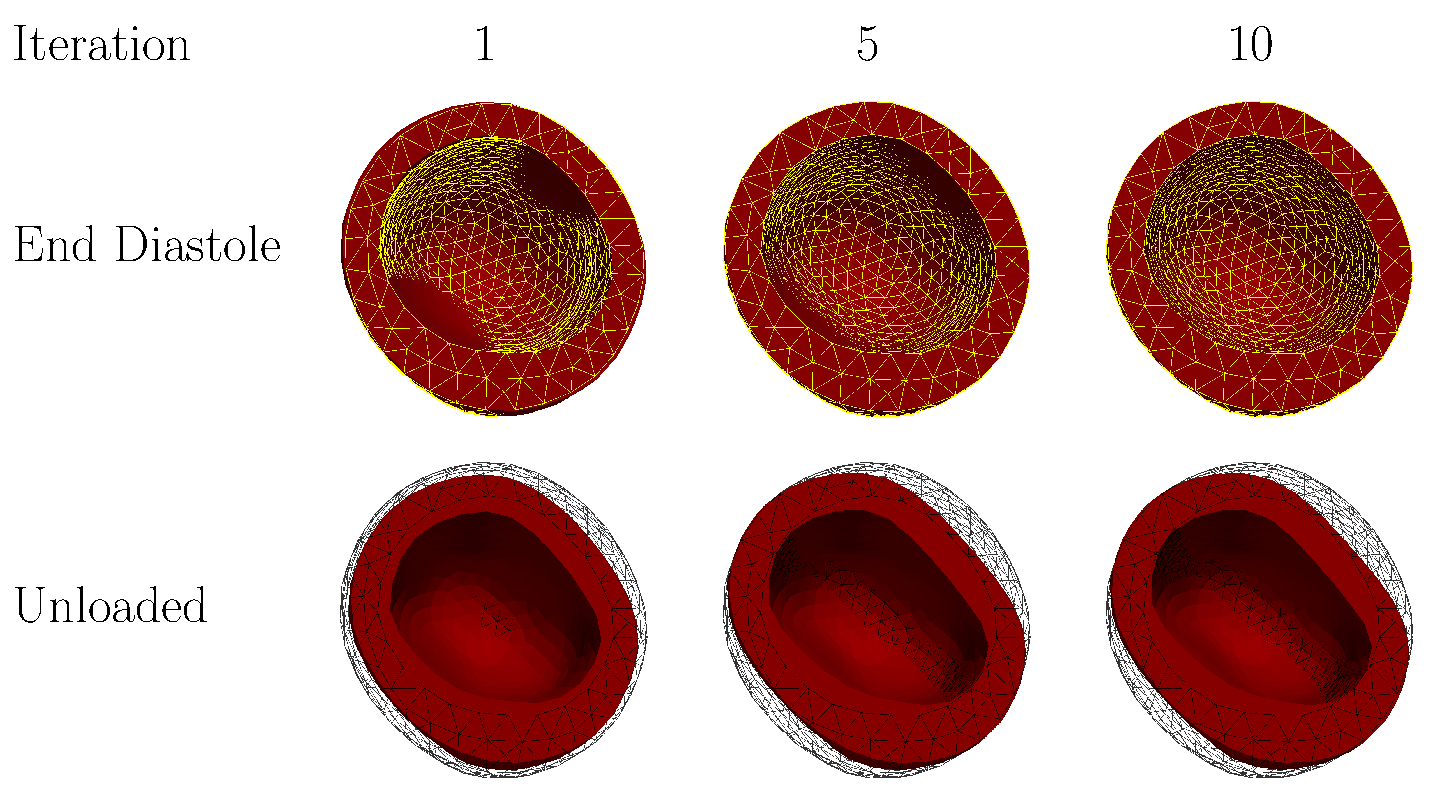
\includegraphics[width=0.9\textwidth]{chapters/introduction/figures/unloading/canvas.pdf}
\caption{Showing 1, 5, and 10 iterations of the backward displacement
  method applied to a left ventricular geometry. To row top shows the
  original geometry in solid and the inflated unloaded geometry in
  yellow wireframe for 1,5 and 10 iterations. Bottom row shows the
  unloaded geometry in solid and the original image based geometry in wireframe.}
\label{fig:unloading_lv}
\end{figure}


Suppose you are given geometry $\Omega_{\mathcal{I}}$ taken from some medical image, and
is thus loaded with some loads $\mathbf{T}$, and we want to find the unloaded geometry
$\Omega_{\mathcal{U}}$, which is so that when we load $\Omega_{\mathcal{U}}$ with $\mathbf{T}$,
you get back the starting geometry $\Omega_{\mathcal{I}}$. Let
$\Xvec_{\mathcal{I}}$ denote the coordinates in $\Omega_{\mathcal{I}}$, and
let $\mathbf{d}$ denote the displacement field which is the solution
of \eqref{some_force_balance_eq} with $\mathbf{T}$ representing
the traction on the endocardium, and which depends on the referece
coordnates. What we want, is to find
$\Xvec_{\mathcal{U}}$ so that $\Xvec_{\mathcal{I}} =
\Xvec_{\mathcal{U}} + \mathbf{d}(\Xvec_{\mathcal{U}})$. To
find fid $\Xvec_{\mathcal{U}}$ we let
\begin{align}
  \Xvec_{n+1} = g(\Xvec_n) =  \Xvec_{\mathcal{I}} - \mathbf{d}(\Xvec_n),
  && \Xvec_0 = \Xvec_{\mathcal{I}}.
\end{align}
According to Banach Fixed Point Theorem, the mapping $g$ has a
fixed-point if $\| \nabla g \|_{\infty} = \| \nabla \mathbf{d}
\|_{\infty} < 1$. This means that as long as the deformation
resulting from the load $\mathbf{T}$ do not result in a stretch that
is more than $100 \%$, this method will converge.

For a transversely isotropic material (or othotropic), the change in
fiber field when going from one geometry to another, has to be
cosidered. The natural thing to do is apply a \emph{Piola
  transformation} to the fibers in the image based geometry: Let
$\F_{n}= \I - \Grad \left(\mathbf{d}(\Xvec_n) \right)$ and left
$\ef^{n} = J^{-1}\F_{n} \ef$ where $\ef$ is the fiber field on
$\Omega_{\mathcal{I}}$. Another way is to regenerate the fibers (see
Section \ref{sec:rule_based_fiber}) using the new unloaded geometry as
input. We will see in the following numverical experiment that non of
these methods gives the desired result.


\begin{figure}[htbp]
  \centering
    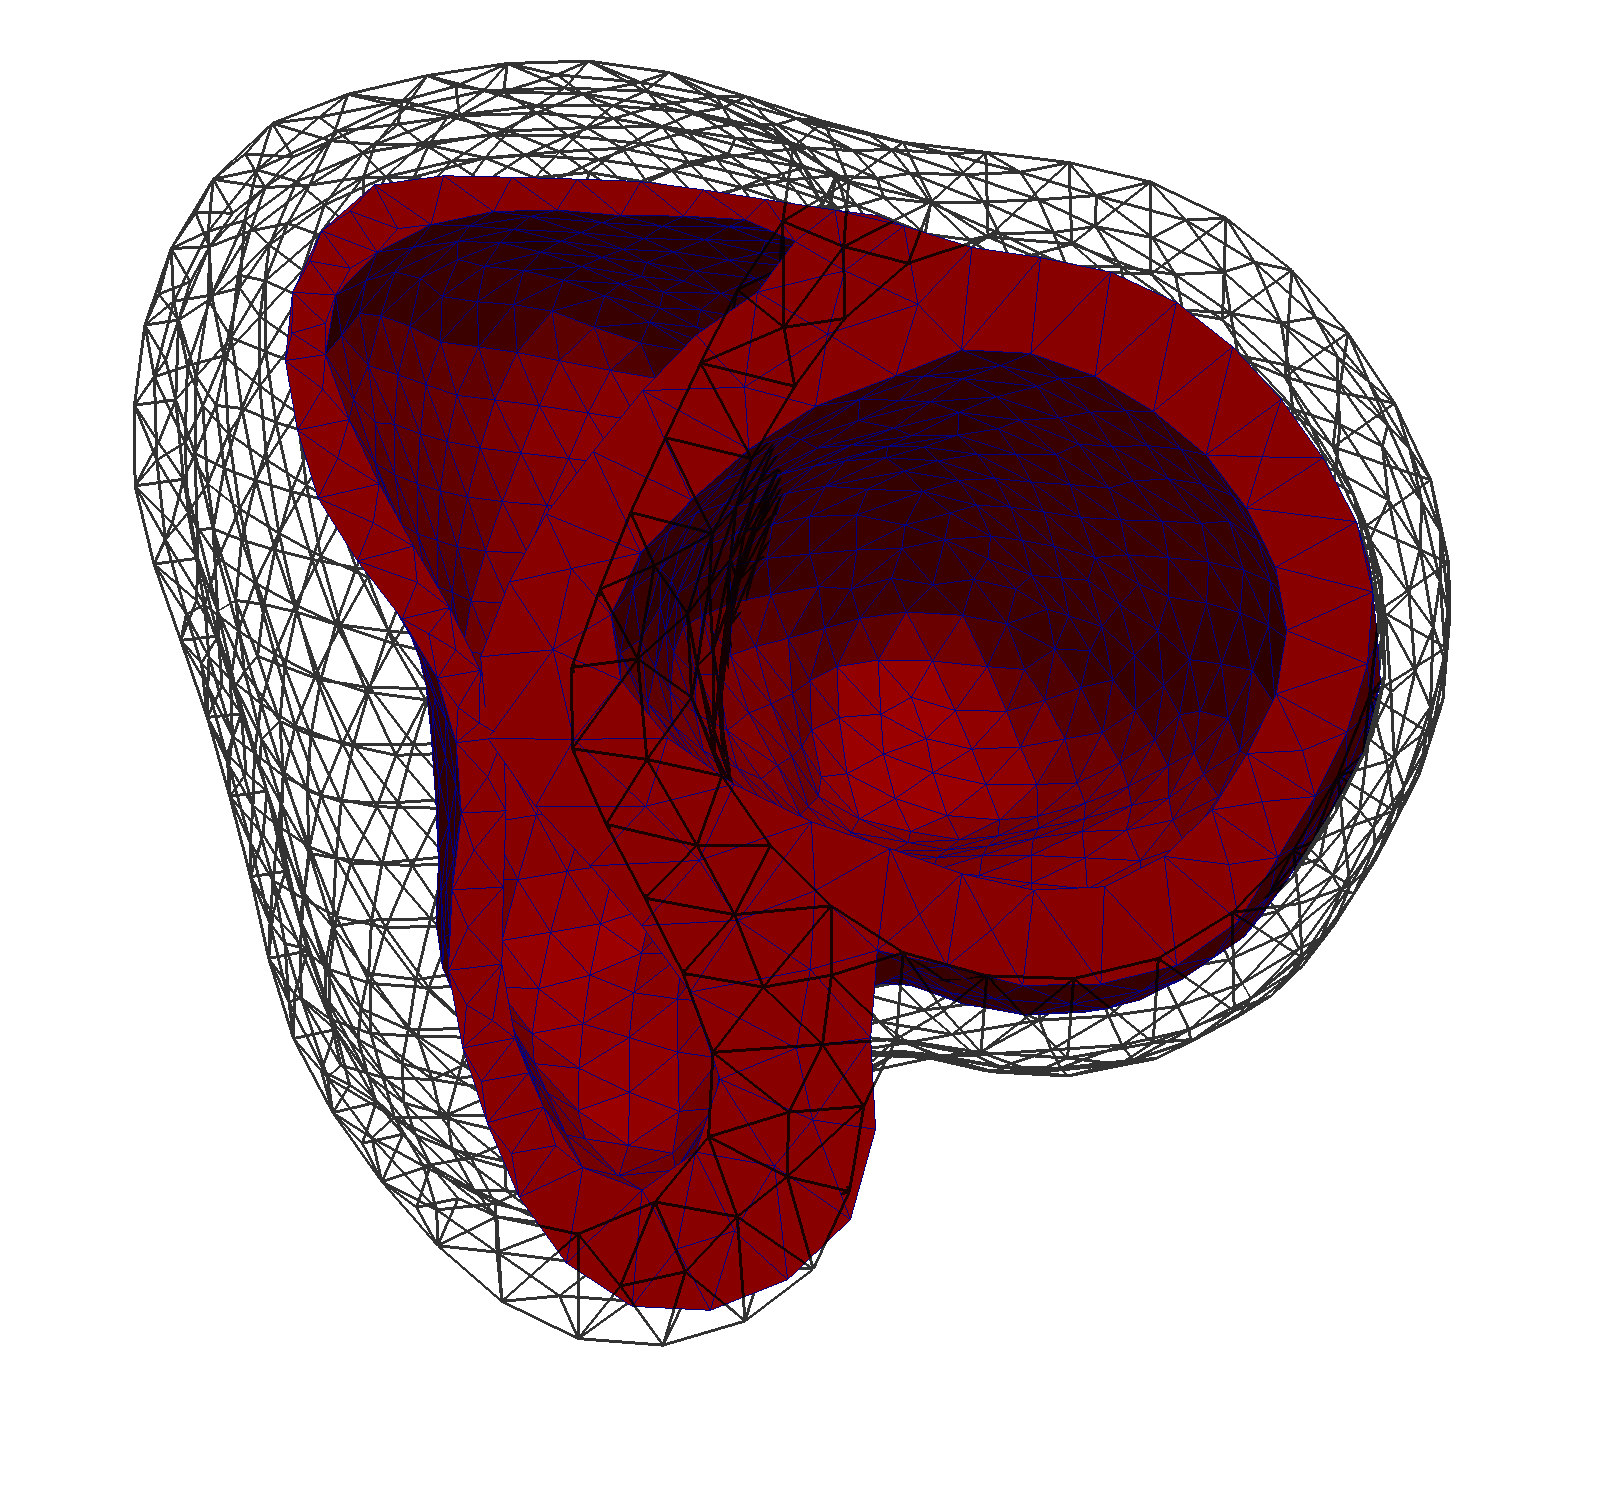
\includegraphics[width=0.5\textwidth]{chapters/introduction/figures/unloading_fail.png}
\caption{Backward displacement method might fail for bi-ventricular
  geometries. This can be seen be noticing that the RV free wall is
  buckling and colliding with the septum.}
\label{fig:unloading_fail}
\end{figure}

\subsubsection{Numerical experiment}
We want to verify that the implementation of the unloading algorithm
behaves as expected. To to this we perform a test where we start with
a known geometry $\tilde{\Omega}_{\mathcal{U}}$ which is our known
unloaded geometry. We inflate $\tilde{\Omega}_{\mathcal{U}}$ to a
pressure $p_{\mathrm{ED}}$, representing the end-diasolic pressure to
get the geometry $\Omega_{\mathcal{I}}$ which will serve as our loaded,
image-based geomtry. The goal is to show that 1) the algorithm is able
to find a geomtry $\Omega_{\mathcal{U}}$ so that when we load it with
the pressure $p_{\mathrm{ED}}$ we get $\Omega_{\mathcal{I}}$ and 2)
the estimated unloaded geometry should converge towards our known
unloaded geometry, in a suitable metric. We choose the directed
Hausdorrf distace \cite{huttenlocher1993comparing} as metric for this
experiment, which is given by
\begin{align}
  d_H(A, B) = \sup_{a \in A} \inf_{b \in B} d(a,b), 
\end{align}
with $d(\cdot, \cdot)$ being the standard euclidean metric. 
The value $d_H(\tilde{\Omega}_{\mathcal{U}}, \Omega_{\mathcal{U}})$
would corresponding to first finding the the closest point in $\Omega_{\mathcal{U}}$ 
for every point in $\tilde{\Omega_{\mathcal{U}}}$, and then taking the
maximum distance between these points. We are interested in two error;
the distance between $\Omega_{\mathcal{I}}$ and the loaded geometry,
and the distance $d_H(\tilde{\Omega}_{\mathcal{U}},
\Omega_{\mathcal{U}})$. To ease notation we refer to these errors as
$d_{\mathcal{I}}$ and $d_{\mathcal{U}}$ respectively.


We test three different cases using the material model in \eqref{eq:holzapel_trans}.
Figure \ref{fig:unloaded_isotropic} shows the error for the case of a
non-linear isotropic materal ($a_f = 0$), and Figure
\ref{fig:unloaded_piola} and \ref{fig:unloaded_regen} shows the case
for a transversely isotropic materail with respectively fibers mapped
via Piola transformation and fibers regenerated at every iteration.
We see that in the isotropic case we are able to recapitulate the
original unloaded geometry as well as in image based geometry, while
in the transversaly isotropic case we are not able to retrieve the
unload correct geometry, and if we regerenete the fibers at each
iteration, the solution start to oscilate. 


% \begin{figure}[htbp]
%   \centering
%   \begin{subfigure}[t]{0.3\textwidth}
%     \includegraphics[width=\textwidth]{numerical_experiments/unloading/unloaded_convergece_iso.png}
%     \caption{\label{fig:unloaded_isotropic}Isotropic}
%   \end{subfigure}
%   \begin{subfigure}[t]{0.3\textwidth}
%     \includegraphics[width=\textwidth]{numerical_experiments/unloading/unloaded_convergece_pushed_fibers.png}
%     \caption{\label{fig:unloaded_piola}Piola transformation}
%   \end{subfigure}
%   \begin{subfigure}[t]{0.3\textwidth}
%     \includegraphics[width=\textwidth]{numerical_experiments/unloading/unloaded_convergece_new_fibers_gen.png}
%     \caption{\label{fig:unloaded_regen}Generate new fibers}
%   \end{subfigure}
% \caption{}
% \label{fig:unloaded_error}
% \end{figure}


\begin{figure}[htbp]
  \centering
    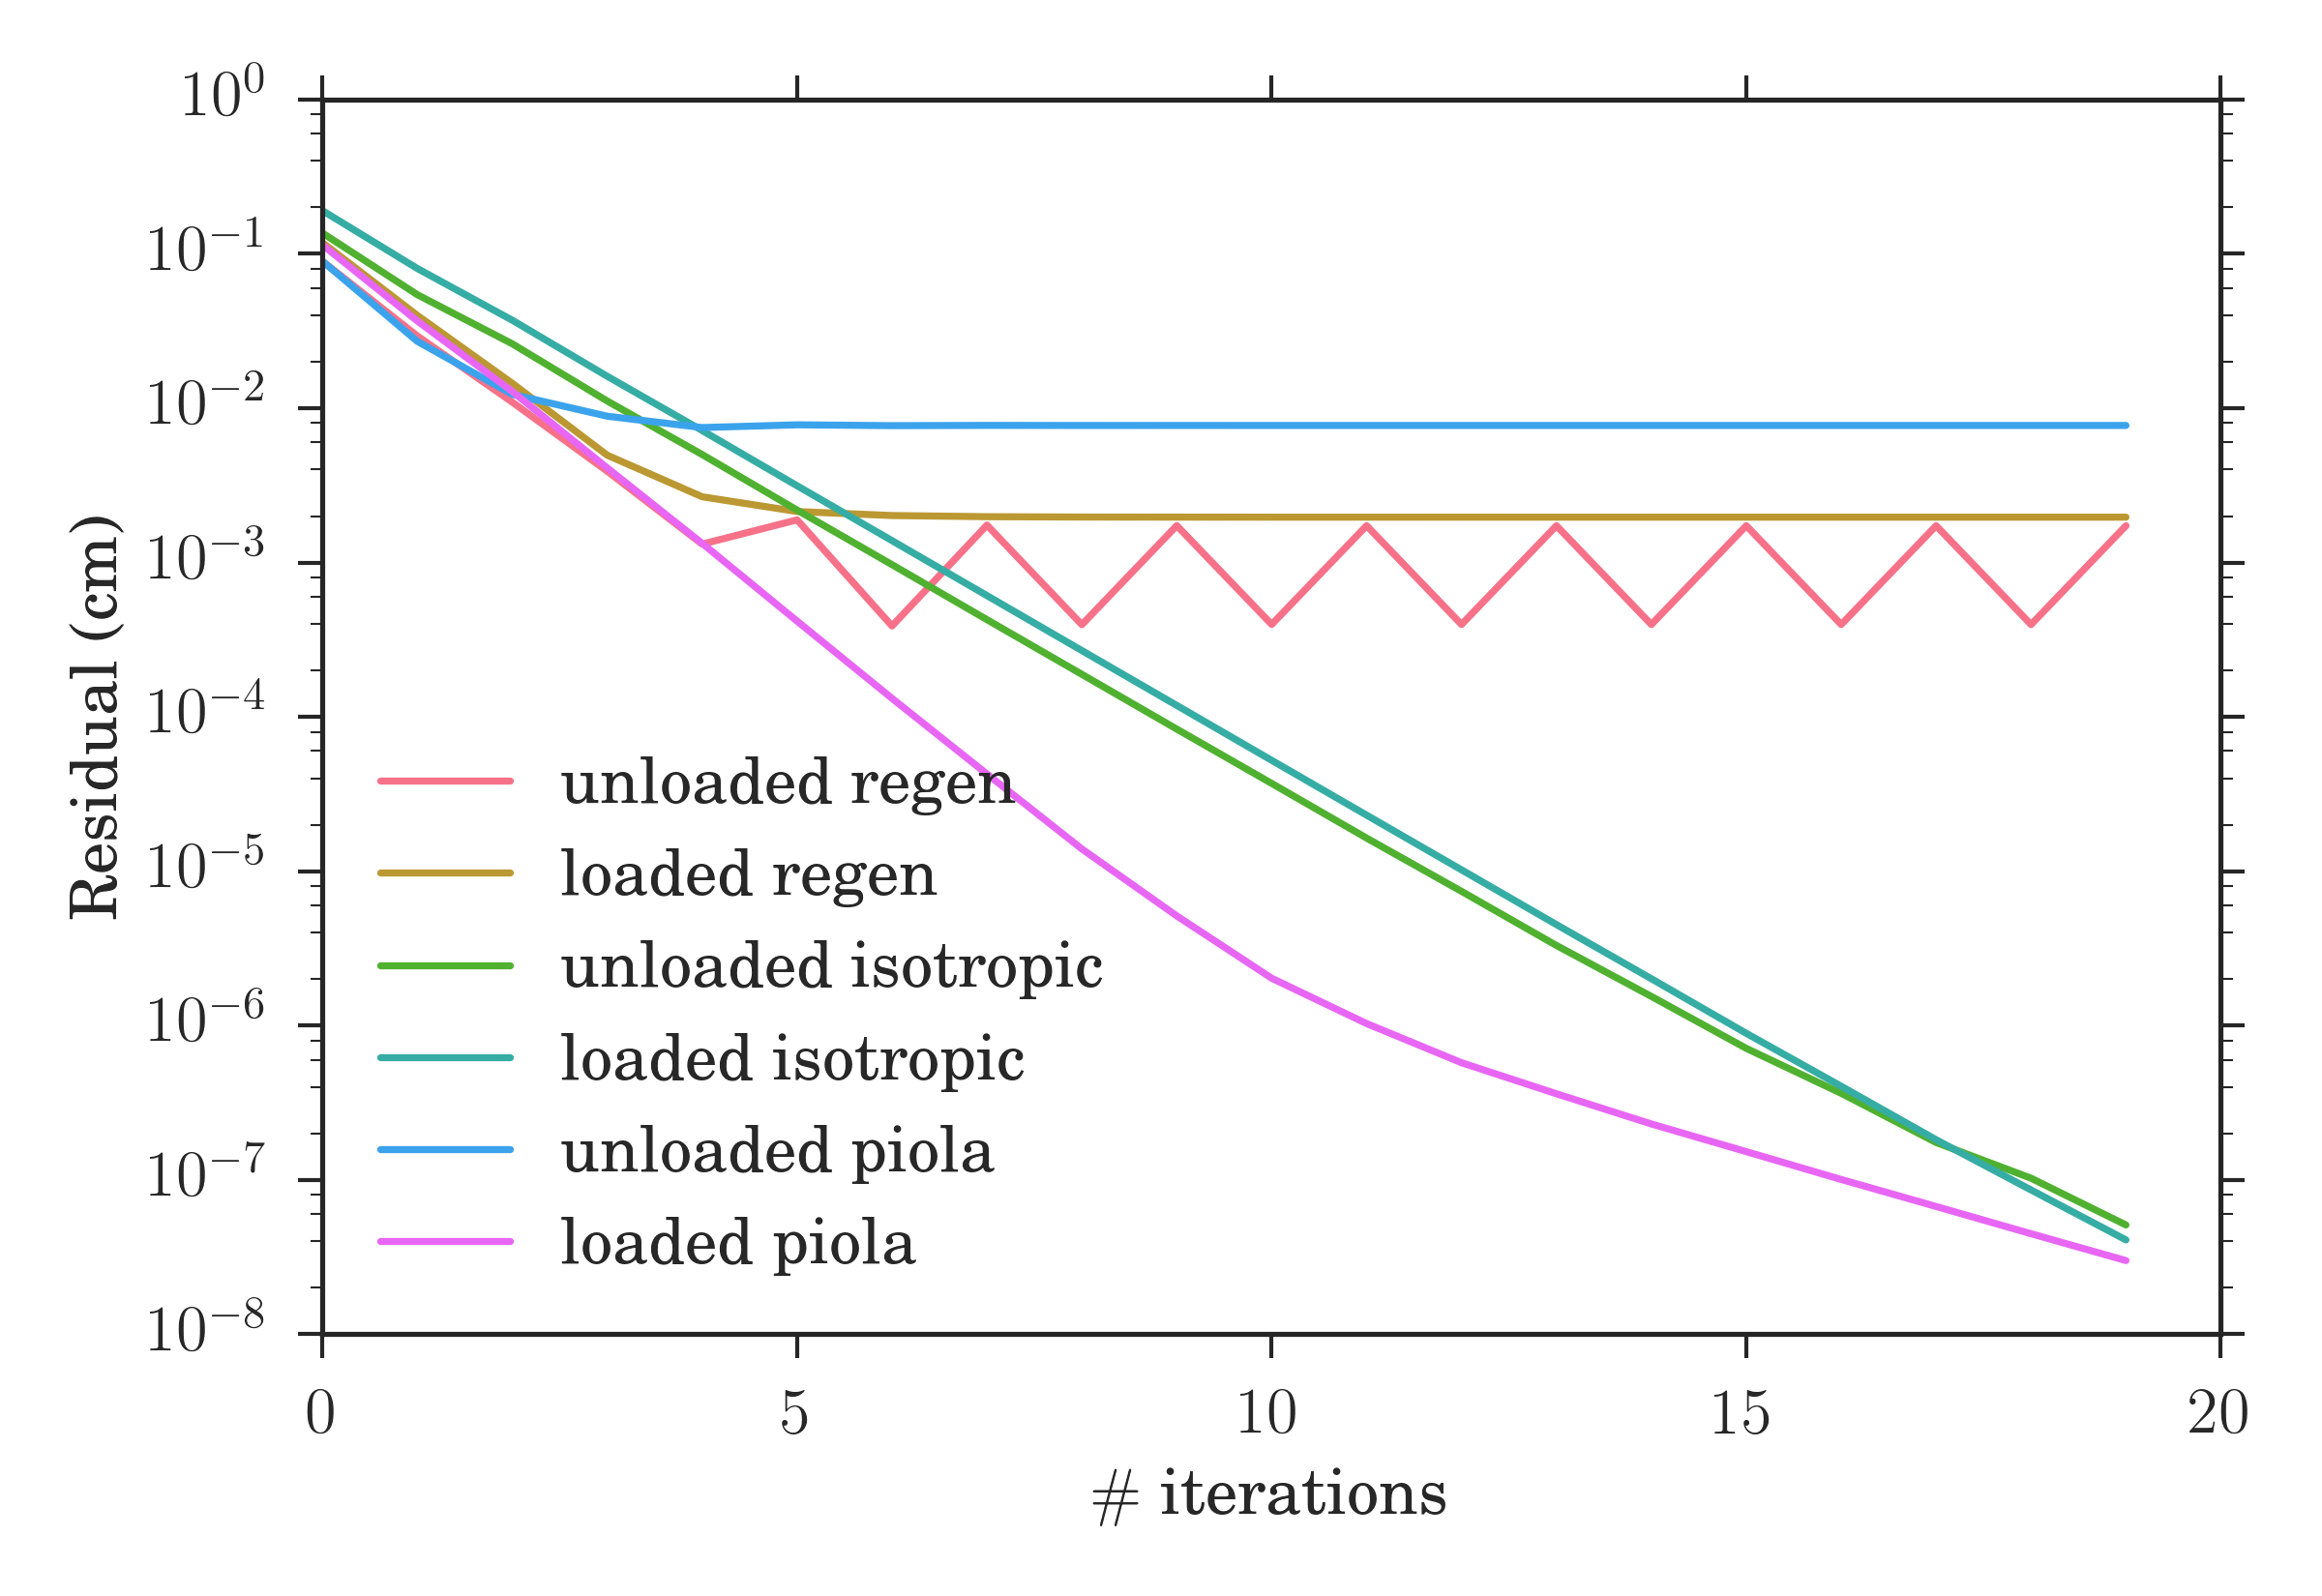
\includegraphics[width=0.7\textwidth]{numerical_experiments/unloading/unloaded_error.png}
\caption{Showing the residual between the known unloaded and estimated
unloaded geometry, and the residual between the loaded geometry and
the image-based geometry. Three differet cases are tested; one where
the material is considered isotropic, one with a transversely
isotropic material with fibers mapped to the new referece geometry via
a Piola transformation, and one with a transversely
isotropic materialwhere the fibers are regenereated at
every iteration. }
\label{fig:unloaded_error}
\end{figure}






\begin{remark}
  The author has observered that when appplying the backward
  displacement method to biventricular geometries subjected to a high
  pressure in the right ventricle, and/or a thin RV free wall, then
  the right ventricluar free wall will in some cases collide with the
  septum. Figure \ref{fig:unloading_fail} shows an example of
  phenomena. In these cases a more robust approach (but less accurate)
  is let $\Xvec_{n+1} = \Xvec_{\mathcal{I}} - k \mathbf{d}(\Xvec_n)$,
  where $\Xvec_n$ is the results from the last converged fixed point
  iteration, and use an optimization algorithm to determine the value
  of $k$ than minimizes some residual. A similar approach has been
  proposed in \cite{raghavan2006non}. 
\end{remark}



\subsection{Implementation details}
A word abour fenics and how we can implement this
Newtons method, good initial guess, increament pressure.
Relatively small system, dense matrix, plot stiffness matrix, Direct
solver.
Fenics compilation stored in cache.
Fibers at quadrature points. Symbolic language.

\subsubsection{FEniCS}
FEniCS is a finite element framework for solving partial differential
equations using a high level of abstraction. The code written in
FEniCS is close to the mathematical notation, and the handling of
assembly code happens ``under the hood'', which makes it easy to use
and intuitive for scientists 

\subsubsection{Numerical considerations}
The solution of non-linear problems such as the one described here is
typically solved using methods like Newton's method. The convergece of
such methods depends on the initial guess, and if the
initial guess is too far from the solution, the solver might diverge.
Moreover, if the initial guess is close to the solution the
convergence rate is in general quadratic.

Let us consider a
typical numerical problem of inflating the ventricular geomtry from a
stress-free configuration to end-diastole. This involves increasing
the pressure, or the boundary tranction on the endocardium, from zero
to the end-diasolic pressure. A strategy know as the
\emph{incremental load} technique is usually a good approach. In this
strategy you select some incremental step-size (for instance $0.4$
kPa), and increase the pressure linearly until the target pressure is
reached. If the solver diverges you decrease the step-size (for
instance by a factor of 0.5) until convergence is reached, and
continue to step up the pressure with the new step-size. This is very
robust, but definetly a slow approach. Since many of the 
constitutive models for myocardium consist of an exponential
realtionship between the stress and strain (so call Fung-type
relation), the amount of stress needed to displace a material will be
higher if the matieral is a state with high strain compared to a state
of low strain. Therefore, the Newtons solver might perform less
iterations to reach convergence when when the load is increased. As a
result, one could improve the incremental load technique by adapting
the step sice if the number of newton iterations are below a certain
threshold (for instance $8$ iterations).

An even more clever strategy, uses a technique from bifurcation
chaos theory and is known as numerical continuation
\cite{allgower2003introduction}.  Suppose we want to
solve the non-linear problem $F(\uvec, \lambda)=0$ with state variable
$\uvec$ and parameter $\lambda$. For instance $\uvec$ could be the
displacement and $\lambda$ could be the endocardial pressure.
The idea be numerical continuations is that given a solution pair
$(\uvec_0, \lambda_0)$ there exist (under conditons stated by the
implicit function theorem) a solution curve $\uvec(\lambda)$ such that
$F(\uvec(\lambda), \lambda)=0$ and $\uvec(\lambda_0) = \uvec_0$.
To explicitly find such a curve is not allways easy but a simple
approximation can be found by extrapolation: Given two pairs
$(\uvec_0, \lambda_0)$ and $(\uvec_1, \lambda_1)$, and a new target
parameter $\lambda_2$, a possible solution is 
\begin{align}
  \uvec_2 =  (1-\delta)\uvec_0 + \delta \uvec_1 && \delta = \frac{\lambda_2 - \lambda_0}{\lambda_1 - \lambda_0}.
\end{align}
% Let $w_0$ denote the initial
% state variable associated with endocardial pressure $p_0$. Increase
% the pressure $p_1 = p_0 + \Delta p_0$, and solve to obtain $w_1$. Next
% we would like to solve for $p_2 = p_1 + \Delta p_1$ where $\Delta
% p_1$ might be the adapted step size. In stead of using $\tilde{w_2}=w_1$ as
% initial guess for the newton solver, as we typically would do in the incremental load
% technique, we observe that if $\delta = \frac{p_2 - p_0}{p_1 - p_0}$,
% and hence $p_2 = (1-\delta)p_0 + \delta p_1$, then a better choice
% of intial guess would be $\tilde{w_2} = (1-\delta)w_0 + \delta w_1$.
Choosing $\uvec_2$ as initial guess for the non-linear solver has been
successfully performed by others in non-linear caridac mechanics
problems \cite{pezzuto2013mechanics}. 


\subsection{Parall Performance}
Write a section here where we test a sample code on multiple cores to
test scalability

Write shorth about MPI, and how mesh is distributed on different
cores in fenics


\begin{table}
  \centering
    \begin{tabular}{llrrrrr}
\hline
   $\#$ elements & Phase & Serial(s) & 1 core (s)& 2 cores (s) &  4 cores (s)&  8 cores (s)\\
\hline
      \multirow{2}{*}{2095} & passive &   26.605 &   26.605 &   20.147 &  12.75 &   7.8642 \\
                      & active &    40.853 &   40.853 &   29.897 &  18.233 &  11.571 \\
      \multirow{2}{*}{8680} & passive & 223.91  &  223.91  &  226.75  & 117.16 &  71.844  \\
                      & active &   190.16  &  190.16  &  193.19  &  99.312 &  60.043 \\
      \multirow{2}{*}{22623} & passive &   1045.1   & 1045.1   & 1248.5   & 571.26 & 337.21   \\
                         & active &   1123.1   & 1123.1   & 1217.1   & 679.88  & 341.71  \\
\hline
    \end{tabular}
    \caption{\label{}Timings running on different number of cores on a
      single node}
  \end{table}


\begin{table}
  \centering
    \begin{tabular}{llrrrrr}
\hline
   $\#$ elements & Phase & Serial (s)& 1 core (s)& 2 cores (s) &  4 cores (s)&  8 cores (s)\\
\hline
      \multirow{2}{*}{2095} & passive &   26.605 &   25.974 &   20.356 &  11.982 &   8.1715 \\
                      & active &   40.853 &   41.061 &   30.028 &  19.922 &  12.482 \\
      \multirow{2}{*}{8680} & passive & 223.91  &  247.74  &  220.68  & 112.04  &  72.954  \\
                      & active &  190.16  &  184.83  &  192.42  &  96.136 &  62.537 \\
      \multirow{2}{*}{22623} & passive &  1045.1   & 1060.6   & 1228.7   & 611.83  & 343.5    \\
                         & active &  1123.1   & 1062.1   & 1268.6   & 597.21  & 364.52  \\
\hline
    \end{tabular}
    \caption{\label{}Timings running on different number of cores
      on two nodes.}
  \end{table}



%%% Local Variables:
%%% mode: latex
%%% TeX-master: "../../main"
%%% End: